%% CauSE 2027 short paper (Position/Short papers: max. 5 pages; ICSE 2027 format = IEEE conference template;
%% double-anonymous; due 13 November 2026 AoE; submit at https://icse2027-cause.hotcrp.com/).
%% compile with: pdflatex main; bibtex main; pdflatex main; pdflatex main
%% Red text (\tbd) is still to be filled in before submission.
\documentclass[10pt,conference]{IEEEtran}

\usepackage{cite}
\usepackage{amsmath}
\usepackage{graphicx}
\usepackage{booktabs}
\usepackage{tabularx}
\usepackage{xcolor}
\usepackage{url}

\newcommand{\tbd}[1]{\textcolor{red}{#1}}
\newcommand{\EAdejumo}[1]{\textcolor{red}{{\bfseries [[#1]]}}}

\begin{document}

\title{Less Tested, Not Worse: The Code-Freeze Rush\\and Soak Time in Kubernetes}

\author{\IEEEauthorblockN{Anonymous Author(s)}}

\maketitle

\begin{abstract}
Large open-source projects ship improvements to their software as new versions, released on a fixed calendar. Kubernetes, which has grown into critical infrastructure for the cloud, publishes such a calendar for each release. In this calendar, there is a period in which code can be merged into the master branch, and a period in which all new work that has not been merged must wait for the next release; this period is called the code freeze. The code freeze triggers a rush, as contributors try to get their code merged before the freeze so that their features ship in the coming release. Crucially, code merged late also reaches users sooner after it is merged, so it spends less time being tested before release. Late code can therefore look worse after release even if it is no worse at all. To investigate how the code freeze shapes when code is merged, and whether late code is worse or only less tested, we analyze 25,579 merged pull requests across 27 Kubernetes releases. We find that on each of the last two days before the code freeze, the number of pull requests approved for merging is three to four times that of an ordinary day. We also see the rush move with the deadline when it was moved. We also find that code merged closer to the code freeze is more likely to need a revert or a fix after release. Additionally, late code is often larger, more often a feature and more heavily reviewed, yet four common explanations, namely the kind of changes that land late, pressure on review, a crowded merge queue and the freeze itself, explain little of this gap. Following each pull request over the same 180-day period after merge, we find that late code shows no excess of problems in total, once we account for the kind of changes that land late. Instead, more of its problems are found after release, and this shift is explained by the shorter duration late code spends on testing before release. We call this duration \emph{soak time}. We discuss what these findings mean for release teams and for studies that count defects after release, and outline future work on testing soak time directly.
\end{abstract}

\begin{IEEEkeywords}
Release engineering, code freeze, causal inference, software defects, Kubernetes, mining software repositories
\end{IEEEkeywords}

\section{Introduction}

In recent years, large open-source projects have moved to time-based releases, shipping on a fixed calendar rather than whenever features are ready~\cite{michlmayr2015timebased}. Kubernetes, the container orchestration system, has shipped three minor releases a year since 2021~\cite{kep2572}. Each release has a \emph{code freeze}: every enhancement for the release must be reviewed and approved by a fixed date, after which only approved changes for the release are merged until the freeze lifts, and the release ships about four weeks later~\cite{k8sphases,k8scycle}. A fixed deadline invites a rush.

The rush is easy to see (Fig.~\ref{fig:rush}). On an ordinary day, about 10 pull requests per release become ready to merge; on the last day before the freeze, 39 do. When the v1.31 freeze was moved two weeks later~\cite{k8s131freeze}, the rush moved with it. Code merged in the rush also appears riskier. The share of pull requests that need a revert or a fix after release rises steadily as the freeze approaches, from 0.35\% for pull requests ready two to three months before the freeze to 1.8\% for those ready in its final 48 hours (Fig.~\ref{fig:changes}a).

The natural reading is that rushed code is worse, and this would not be new to software engineering. Changes committed on Fridays~\cite{sliwerski2005fridays} or late at night~\cite{eyolfson2011time} were found to induce fixes more often, and time pressure has been linked to lower quality and skipped quality assurance~\cite{kuutila2020time}.

These studies ask whether the timing of a change affects \emph{how often} it fails. A separate question is whether timing affects \emph{when} failures appear. At the release level, faster release cycles were found to change when users encounter bugs, but not how many they encounter~\cite{khomh2012faster}. For a single change, the time between merge and release may matter in the same way. Kubernetes treats this time as a period of testing and stabilization~\cite{k8scycle}, and the weeks before release focus on ``fixing bugs, eliminating test flakes and general release stabilization''~\cite{k8sphases}. Code merged late spends less of this time on the master branch before it reaches users. We therefore ask whether merging late moves a failure from before the release to after it. In causal terms, when the outcome window starts at the release, the time until release may act as a mediator: merging late (the treatment) shortens this time, which could make a post-release problem (the outcome) more likely even if the code is no worse.

Using 25,579 pull requests across 27 Kubernetes releases (v1.11--v1.37), we first describe how the code freeze shapes when code is merged, and how merging close to the freeze relates to problems after release. We then test four common explanations for the gap, and finally follow every pull request for the same period from merge, to see whether late code fails more often or is simply found failing later. We find that: (1)~The rush is concentrated in the final 48 hours, moves when the deadline moves, and has grown since 2021; problems after release rise steadily as the freeze approaches, and pull requests ready in the final week are 2.5 times as likely as earlier ones to have one. (2)~Late pull requests are larger, more often features and more heavily reviewed, yet none of four common explanations accounts for more than about one in twenty of the gap. (3)~Problems in late and early code surface equally fast after merge, but late code reaches the release sooner: a pull request merged in the final week gets about one month of testing before release, while one ready two to three months before the freeze gets about three. We call this time \emph{soak time}. When we follow every pull request for the same 180 days after merge and account for the kind of changes that land late, we see no sign that late code has more problems in total. But more of its problems are found after release, which is in line with its shorter soak time.

We make the following contributions:
\begin{enumerate}
\renewcommand{\labelenumi}{\roman{enumi}.}
\item \textbf{A detailed picture of the code-freeze rush:} We show how the rush builds day by day, follows the deadline, and has grown across 27 releases, and how problems after release rise as the freeze nears.
\item \textbf{Preliminary evidence that the late-merge gap is soak time:} In Kubernetes, late code is less tested before release, not worse: four common explanations account for little of the gap, while soak time predicts the share of problems found after release.
\item \textbf{A timing view of post-release defects:} We show that counting defects after release mixes how often code fails with when failures are found, and that following every change for the same window from merge separates the two.
\end{enumerate}

\begin{figure*}[t]
\centering
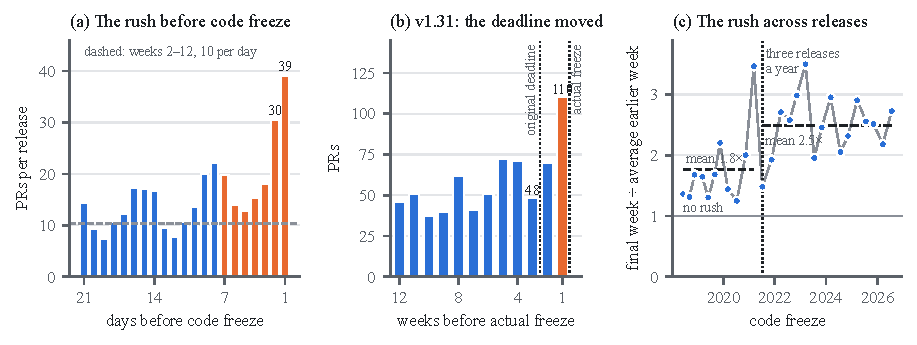
\includegraphics[width=\textwidth]{figures/fig_rush.pdf}
\caption{The code-freeze rush in Kubernetes. (a) Pull requests per release by the day they became ready to merge, over the final three weeks before code freeze (27 releases, v1.11--v1.37); orange marks the final week. (b) v1.31 pull requests by week: the freeze was moved two weeks later, from the original deadline to the actual freeze. (c) Pull requests in each release's final week, divided by an average earlier week; dashed lines are the means before and after the move to three releases a year.}
\label{fig:rush}
\end{figure*}

\section{Background \& Related Work}

\textbf{The Kubernetes release cycle.} A pull request to Kubernetes merges only after a reviewer applies the \texttt{lgtm} label and an approver applies the \texttt{approved} label; a merge bot then merges labeled pull requests once their tests pass. Before code freeze, every enhancement for the release must carry both labels, and because merges wait in a queue, approved pull requests may merge shortly after the deadline~\cite{k8sphases}. After the freeze, the release team accepts late enhancements only as exceptions, which should be ``well-tested'' and low risk~\cite{k8sphases}. The project describes its release process as ending in a \emph{stabilization} phase, and the roughly two weeks between the end of code freeze and the release are for resolving ``all remaining critical issues''~\cite{k8scycle}. Release engineering research has long argued that such processes shape software quality~\cite{adams2016release}.

\textbf{Timing and defects.} Śliwerski et al. found that changes committed on Fridays were more likely to induce fixes~\cite{sliwerski2005fridays}, and Eyolfson et al. found that commits made late at night were buggier~\cite{eyolfson2011time}. Time pressure more broadly has been linked to lower quality and skipped quality assurance~\cite{kuutila2020time}. At the level of releases, Khomh et al. found that after Firefox moved to rapid releases, users met bugs earlier and bugs were fixed faster~\cite{khomh2012faster}, and Mäntylä et al. showed that shorter release cycles change how much and what kind of testing happens before release~\cite{mantyla2015rapid}.

\textbf{Measuring problems.} Defect studies often link a fix back to the change that introduced it~\cite{sliwerski2005changes}, an approach whose links are known to be noisy~\cite{dacosta2017framework,rosa2021szz}, and many count the defects found in a window after release~\cite{zimmermann2007predicting}. Reverts are a second signal: a revert removes a change, often but not always because it broke something~\cite{shimagaki2016reverted}. Review coverage and participation have been related to such post-release defects~\cite{mcintosh2014review}.

\textbf{Causal methods in software engineering.} Causal inference is increasingly used in software engineering~\cite{siebert2023causal}. We follow the potential-outcomes view~\cite{hernan2020causal}, use doubly robust estimation~\cite{bang2005doubly}, and treat merge-queue load as an exposure under interference~\cite{aronow2017interference}.

Building on these works, we ask the following research questions:

\noindent\textbf{RQ1} \textit{How does the code-freeze rush unfold, and how does it relate to problems after release?}

\noindent\textbf{RQ2} \textit{Does late code fail more often, or are its failures found later?}

\section{Methodology}

\subsection{Dataset Selection}
We collected every pull request merged into \texttt{kubernetes/kubernetes} for 27 releases, v1.11 to v1.37, whose code freezes fall between June 2018 and July 2026. We applied the following criteria:
\begin{enumerate}
\renewcommand{\labelenumi}{\roman{enumi}.}
\item \textbf{Release calendar:} For each release, we took the date and time of its code freeze and the date of its release from the release team's published schedule~\cite{k8sschedules}. For v1.31, whose freeze was moved, we use the new date.
\item \textbf{Readiness:} Because the merge queue can delay a merge past the deadline, we date each pull request by its \emph{readiness}, the later of the times its \texttt{lgtm} and \texttt{approved} labels were applied before merge. We rebuilt each label history from the pull request's timeline and checked it by replaying the history against the labels the pull request carries today.
\item \textbf{Window:} We keep pull requests that became ready within 12 weeks before a code freeze, and assign each to that release. Pull requests ready in the final 7 days are \emph{late}; those ready 2 to 12 weeks before are \emph{early}. We exclude pull requests opened by bots.
\end{enumerate}
Thus, our population has 25,579 pull requests, 4,035 of them late.

\subsection{Identifying Problems}
We say a pull request had a \emph{problem} when it was later reverted or fixed. We use ``problem'' rather than ``bug'' because a revert shows that a change was pulled out, not always that it was faulty.

\textbf{Reverts:} We first find revert pull requests: those whose title starts with ``Revert'' or whose branch was created by GitHub's revert button. We then link each revert to the pull request it undoes, using any one of three clues: the original's pull request number in the revert's title, branch name or description; the original's title quoted in the revert's title; or the commit recorded by \texttt{git revert}. Finally, we check that the revert undoes the original: it must change at least one of the original's files with the additions and deletions swapped. We keep only the reverts that pass this check.

\textbf{Fixes:} A fix is a later pull request that references the original by number. Pull requests reference each other for many reasons, so we keep only fixes that use words such as ``regression'', ``broke'' or ``introduced in'', and that change at least one file the original changed. One author then hand-coded every such link that falls inside our outcome windows, answering whether the second pull request fixes a defect introduced by the first. The coding page showed both pull requests' titles, descriptions, labels and changed files in random order, but not their dates or whether the original was late. We keep only the links coded as fixes, and count links the author could not decide as not fixes.

Our analysis plan, fixed before estimation, counted every revert or referencing link. For RQ1 and the four explanations in RQ2, we report those planned results and repeat every test on verified reverts and hand-confirmed fixes (\emph{hand-checked} problems); for the soak time analysis, we use the hand-checked problems. Since we only count problems that someone linked back to a pull request, our counts should be interpreted as lower bounds.

\subsection{How does the code-freeze rush unfold? (RQ1)}
\textbf{The rush:} For each release, we count the pull requests that became ready on each day before its freeze. We then compare the last days before the freeze with an ordinary day 2 to 12 weeks earlier. To measure the size of the rush in each release, we divide the number of pull requests in the final week by the number in an ordinary earlier week. We also ask whether the rush grew when Kubernetes moved to three releases a year (v1.22). We compare the share of late pull requests before and after this move with a regression weighted by release size, which also accounts for how far into the cycle the freeze fell. Finally, in v1.31 the release team moved the freeze two weeks later, from 10 to 24 July 2024, and announced this on 28 June~\cite{k8s131freeze}. We compare the week before the original deadline with the week before the new one.

\textbf{The impact:} We place each pull request in a group by how long before the freeze it became ready: 9--12 weeks, 5--8 weeks, 3--4 weeks, week 2, days 3--7, or the final 48 hours. Our main outcome is whether a pull request had a problem found in the 90 days after its release. Because every pull request in a release ships on the same day, this window covers the same dates for all of them. We also count two outcomes measured from merge: a revert within 30 days, and a fix within 30 days. To compare late and early pull requests, we use the risk ratio: how many times as likely a late pull request is to have a problem. Pull requests in the same release share its release date and conditions, so our confidence intervals allow for this (clustered by release). Finally, we repeat the comparison with a fake deadline six weeks before the real freeze (a placebo): if the gap comes from the deadline, it should not appear there.

\textbf{What changes as the freeze nears:} Using the same six groups as above, from 9--12 weeks before the freeze to its final 48 hours, we describe what the pull requests in each group look like: their size (lines changed), their kind (the share labeled as features), how much review they received (review threads), how experienced their authors are (the author's prior pull requests), and how long they wait on the master branch before release (days from merge to release). Apart from the problem rates by group and the test of the cadence change, which were planned, the series in Figs.~\ref{fig:rush} and~\ref{fig:changes} were added after seeing the results.

\subsection{Does late code fail more often, or are its failures found later? (RQ2)}
Late pull requests may have more problems after release than early ones; we call this difference \emph{the gap}. We test four common explanations for it, each set out in our plan before we estimated any effects, and we report all four. Three of them say that late code is worse: it may be a different kind of change (composition), it may be reviewed less carefully (pressure on review), or it may break when merged alongside many other changes (a crowded merge queue). The fourth says that the freeze changes how problems are handled: a problem found during the freeze may be reverted rather than fixed (freeze response). Finally, we test a fifth explanation, added after seeing the first four results: late code is no worse, but has less time to be tested before release (soak time).

\textbf{What lands late (composition):} Larger changes are more likely to introduce defects; the number of lines a change adds remains one of the strongest predictors of whether it does~\cite{kamei2013jit,zeng2021deep}. If the changes that land late differ from those that land early, for example in size or kind, a difference in problems may come from what lands late, not from when it lands. We reweight early pull requests (5 to 12 weeks before the freeze) to match late ones on size label, lines and files changed, kind labels, number of SIGs, milestone, priority, the author's prior pull requests, the pull request's age and its release, using inverse-probability weights and a doubly robust estimator, with a bootstrap over releases (400 replicates). The share of the gap removed by reweighting is the share explained by composition.

\textbf{Pressure on review:} Under time pressure, developers tend to cut back on quality assurance~\cite{kuutila2020time}, and how a change is reviewed has been linked to whether it introduces defects~\cite{mcintosh2014review,thongtanunam2021review}. Reviewers facing the deadline may approve late pull requests with less scrutiny. We compare late and early pull requests by the same author (author fixed effects), and estimate the share of the gap that runs through four review measures: review threads, reviews, whether \texttt{lgtm} was removed, and time from the last commit to readiness.

\textbf{A crowded merge queue (congestion):} When many changes merge at once, changes developed in parallel can conflict and break the build~\cite{dasilva2022build}, even when each passes its tests alone~\cite{ananthanarayanan2019keeping}. A deadline packs merges into its final days, and so may raise this risk. Within the final week, holding the time to freeze fixed in 6-hour bins, we relate problems to the number of pull requests merged in the same area within 12 hours, total merges within 6 hours, and queue wait. Congestion is supported only if the same relation also appears in weeks 2 to 12, where there is no deadline.

\textbf{The freeze itself (freeze response):} During the freeze, only changes for release-blocking issues may merge~\cite{k8sphases}, so a change that causes trouble may be reverted to protect the release where it would otherwise be fixed forward. Reverting is a common way to recover from a problematic change, and reverts are also made for reasons other than defects~\cite{shimagaki2016reverted,yan2019reverted}. Among pull requests with a problem within 30 days of merge, we test whether problems that surfaced during the freeze were more often reverted than fixed forward, holding composition fixed.

\textbf{Less time before release (soak time):} We added this explanation after seeing the results of the first four. Those four ask whether late code is worse or handled differently; none asks \emph{when} its problems are counted. Our main outcome counts problems from the release onward. Since every pull request in a release ships on the same day, one merged late spends less time on the master branch before release. We call this time \emph{soak time}. Kubernetes treats it as a period of testing and stabilization~\cite{k8scycle,k8sphases}, and the release cycle is known to change how much testing happens before release~\cite{mantyla2015rapid} and how long finished work waits to reach users~\cite{dacosta2018integration}. A problem that would be caught before release in an early pull request may therefore be caught only after release in a late one, so late code could show more problems after release without being worse. To test this, we follow every pull request for the same 180 days from merge, regardless of when its release ships, and record whether its first problem was found before or after release. This window is long enough for every pull request to reach its release, with time left after it: we include pull requests ready up to 12 weeks before the freeze, and releases ship within seven weeks after it. A shorter window, such as 90 days, would end before the release for many early pull requests, so none of their problems could be found after release. If late code is worse, it should have more problems in total. If it is only less tested, the total should be the same, but more of its problems should be found after release. We repeat the reweighting and same-author comparisons above for all problems, for those found before release, and for those found after. Next, we compare how fast problems surface after merge in late and early code, as the share found within each number of days. If they surface equally fast, the time to release alone decides how many are found after it. Finally, we compute this expected share: we take the early pull requests' discovery times (days from merge to first problem) and count how many would fall after each late pull request's release. We repeat this for each week before the freeze, each time using the discovery times of the other weeks.

\section{Preliminary Findings}

\subsection{How does the code-freeze rush unfold? (RQ1)}

\textbf{The rush:} On an ordinary day 2 to 12 weeks before the freeze, about 10 pull requests per release become ready to merge. In the final week this rises, and on the last two days it reaches 30 and 39 (Fig.~\ref{fig:rush}a): the final 48 hours alone carry about 70 pull requests per release. The rush is driven by the deadline itself. When the v1.31 freeze was moved two weeks later, twelve days before the original deadline, the week before that deadline brought only 48 pull requests, while the week before the new one brought 110, the most of any week in that release (Fig.~\ref{fig:rush}b). The rush has also grown. Before 2021, the final week brought 1.8 times as many pull requests as an average earlier week; since the move to three releases a year, it brings 2.5 times as many (Fig.~\ref{fig:rush}c), and the share of late pull requests rose by 5.2 percentage points [2.5, 8.0].

\begin{figure*}[t]
\centering
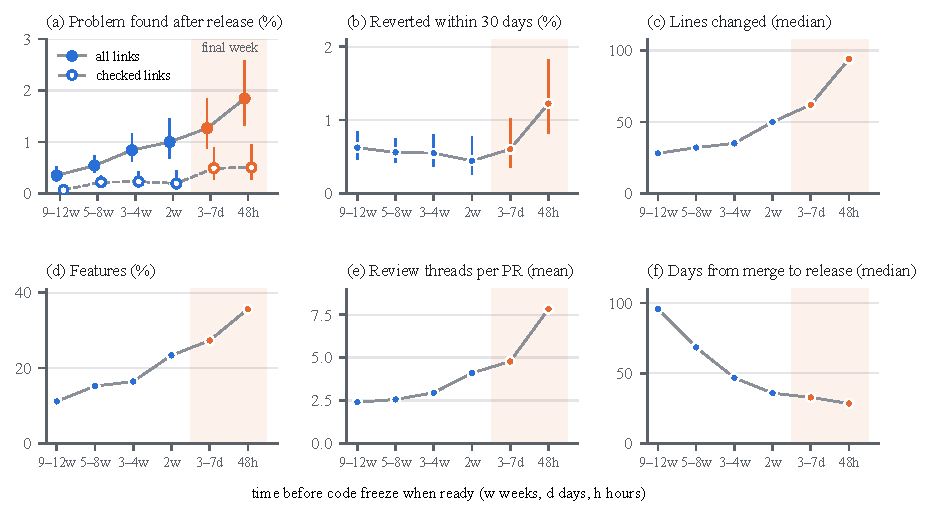
\includegraphics[width=\textwidth]{figures/fig_changes.pdf}
\caption{How pull requests change as the freeze approaches, grouped by the time before code freeze at which they became ready (shaded: the final week). (a) Share with a problem found in the 90 days after release, for all links and for hand-checked problems. (b) Share reverted within 30 days of merge (verified reverts). (c--f) Lines changed, share of features, review threads, and days from merge to release. Bars are 95\% confidence intervals.}
\label{fig:changes}
\end{figure*}

\textbf{The impact:} The closer to the freeze a pull request became ready, the more likely it was to have a problem found after release (Fig.~\ref{fig:changes}a). The share rises steadily from 0.35\% for pull requests ready 9 to 12 weeks before the freeze, through 0.84\% for weeks 3 to 4, to 1.26\% for days 3 to 7 and 1.84\% for the final 48 hours. Hand-checked problems show the same rise at a lower level, from 0.06\% to 0.50\%. Overall, 1.5\% of late pull requests and 0.6\% of early ones had a problem found after release, a risk ratio of 2.55 [1.93, 3.38]; on hand-checked problems, the ratio is 2.93 [1.74, 4.95]. A placebo deadline six weeks before the freeze shows no such gap (0.71 [0.38, 1.33]). The gap did not clearly grow with the rush after the move to three releases a year (+0.2 percentage points [$-0.6$, 0.9]; +0.6 [0.2, 1.0] on hand-checked problems), and v1.31 had too few problems to compare its two deadline weeks (one each).

Reverts behave differently (Fig.~\ref{fig:changes}b). The share reverted within 30 days of merge stays between 0.4\% and 0.6\% from 12 weeks before the freeze until its final 48 hours, then doubles to 1.2\%. Overall, late pull requests were more often reverted within 30 days (1.57 [1.09, 2.26]), but not more often fixed within 30 days (1.28 [0.98, 1.67]; on hand-checked problems, 1.03 [0.54, 1.95]).

\textbf{What changes as the freeze nears:} From 9--12 weeks before the freeze to its final 48 hours, pull requests grow larger (a median of 28 to 94 lines changed), are more often features (11\% to 36\%) and receive more review (2.4 to 7.8 review threads), while their authors are equally experienced and the time before release falls from a median of 96 to 28 days (Fig.~\ref{fig:changes}c--f).

\subsection{Does late code fail more often, or are its failures found later? (RQ2)}

\begin{table}[t]
\caption{Candidate explanations for the gap in problems found after release. Planned: all links, as pre-specified. Checked: verified reverts and hand-confirmed fixes. pp: percentage points; 95\% CIs in brackets.}
\label{tab:explanations}
\centering
\footnotesize
\setlength{\tabcolsep}{2.5pt}
\begin{tabularx}{\columnwidth}{@{}>{\raggedright\arraybackslash}Xllc@{}}
\toprule
Explanation (test) & Planned & Checked & Explains? \\
\midrule
The gap: late vs early (risk ratio) & 2.55 [1.93, 3.38] & 2.93 [1.74, 4.95] & -- \\
What lands late: share of the gap removed by reweighting & 1.2\% [$-6.7$, 9.4] & 0.5\% [$-29.1$, 19.1] & No \\
Pressure on review: gap within the same author (pp) & 1.09 [0.63, 1.54] & 0.34 [0.10, 0.59] & \\
\quad through review measures (pp) & 0.06 [0.02, 0.10] & 0.01 [$-0.02$, 0.03] & No \\
Crowded queue: same-area merges per IQR, final week (pp) & 0.66 [0.06, 1.25] & 0.40 [$-0.09$, 0.89] & \\
\quad same, weeks 2--12 (pp) & 0.03 [$-0.15$, 0.22] & 0.03 [$-0.09$, 0.16] & No \\
Freeze response: reverted rather than fixed, in vs out of freeze (pp) & 3.0 [$-6.6$, 12.6] & 5.9 [$-7.6$, 19.4] & No \\
\bottomrule
\end{tabularx}
\end{table}

\textbf{Candidate explanations:} None of the four common explanations accounts for the gap, with either set of links (Table~\ref{tab:explanations}). The kind of changes that land late explains about 1\% of it: although late pull requests are larger and more often features, reweighting early pull requests to look like late ones leaves the gap almost unchanged. Pressure on review does not explain it either. The gap remains for the same author (+1.09 percentage points), and only about one in twenty of it runs through review; in fact, late pull requests receive more review, not less. A crowded queue shows a weak relation in the final week for merges in the same area, but no relation in weeks 2 to 12, so it does not meet our test for congestion. Finally, problems that surface during the freeze are not more often reverted (22.7\% vs 20.8\%; adjusted +3.0 percentage points [$-6.6$, 12.6]). Reweighting does, however, absorb much of the 30-day revert gap, which halves and can no longer be told apart from zero (+0.15 percentage points [$-0.31$, 0.48]).

\textbf{Total vs timing:} Followed for 180 days from merge, 2.1\% of late and 1.5\% of early pull requests had a problem. Once the kind of changes that land late is taken into account, the difference is $-0.2$ percentage points [$-1.6$, 0.7]: we find no sign that late code has more problems in total. The timing of those problems, however, differs. Late pull requests had more problems found after release (0.47\% vs 0.18\%; adjusted +0.33 percentage points [0.17, 0.50]), and, after adjustment, slightly fewer found before release ($-0.5$ [$-2.0$, 0.6]). The pattern holds for the same author (after release +0.32 [0.09, 0.54]) and with all links (total +0.76 [$-0.49$, 1.83]; after release +1.15 [0.78, 1.50]).

\begin{figure*}[t]
\centering
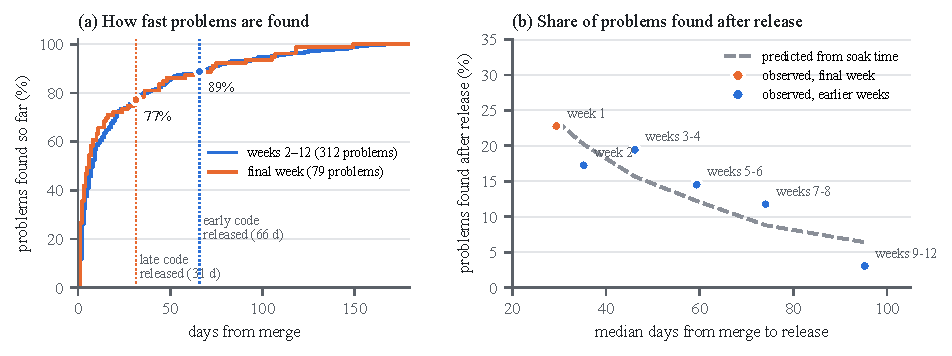
\includegraphics[width=\textwidth]{figures/fig_soak.pdf}
\caption{Soak time. (a) Share of problems found within a given number of days of merge, for late (final week) and early (weeks 2--12) pull requests; dotted lines mark the median days from merge to release, and the dots the share already found by then. (b) Share of each week's problems found after release, against the median days from merge to release. The dashed line is the share predicted from soak time alone, using the other weeks' discovery times. Problems are verified reverts and hand-confirmed fixes within 180 days of merge.}
\label{fig:soak}
\end{figure*}

\textbf{Discovery speed:} Problems in late code surface as fast as problems in early code (Fig.~\ref{fig:soak}a). In both groups, 72\% of problems are found within 21 days of merge, and 87 to 88\% within 60 days; in the first week, late code's problems are, if anything, found slightly sooner (58\% vs 50\%). What differs is when the release comes. Late code ships a median of 31 days after merge, when 77\% of its problems have been found; early code ships after 66 days, when 89\% have.

\textbf{Timing prediction:} Soak time predicts the shift. Given early pull requests' discovery times, 24\% of late pull requests' problems should be found after release, and we observe 23\%; for early pull requests, the prediction is 11\% and we observe 12\%. Across the weeks before the freeze, the observed share falls as soak time grows, from 23\% in the final week to 3\% in weeks 9 to 12, and stays within four percentage points of the prediction in every group (Fig.~\ref{fig:soak}b). The steady rise in problems after release in Fig.~\ref{fig:changes}a, which begins two to three months before the freeze, long before any rush, is the pattern soak time predicts: a gradual rise as the time to release shrinks, rather than a jump at the deadline. In other words, late code appears less tested before release, not worse.

\section{Discussion}

\textbf{The shape of the rush:} The code-freeze rush in Kubernetes is real, concentrated in the final two days, and growing: since the move to three releases a year, the final week brings two and a half times as many pull requests as an ordinary week. The v1.31 freeze, moved two weeks later, shows that the deadline itself drives the rush, which followed the new date. Such series are cheap to compute from a project's history, and they let release teams see how their calendar shapes when work arrives.

\textbf{Less tested, not worse:} Our findings suggest that the extra problems users meet after a release come from less testing time, not from worse code. This matters for what release teams do about the rush. Discouraging late merges is unlikely to work: in v1.31 the rush followed the deadline, so a deadline will always have a final week. What release teams can set is how long the final week's code runs before release. A longer gap between freeze and release, or extra soak for final-week merges, targets the cause. The Kubernetes exception process already asks that late changes be ``well-tested''~\cite{k8sphases}; soak time offers a measurable version of that request. One signal does peak at the deadline: pull requests ready in the final 48 hours are reverted within 30 days twice as often. These are the largest pull requests and most often features, and once the kind of changes that land late is taken into account, the final week's revert gap can no longer be told apart from zero.

\textbf{Time pressure and review:} Time pressure has been linked to lower quality and skipped quality assurance~\cite{kuutila2020time}. In Kubernetes, late pull requests received more review, not less, with three times as many review threads in the final 48 hours as two to three months before the freeze. This suggests that the project's review process absorbs much of the rush, and that the remaining risk lies in what review cannot catch: problems that only show up after code has run for a while.

\textbf{Counting defects after release:} Many studies count defects in a window after release~\cite{zimmermann2007predicting}, and others relate the timing of a change to its defects~\cite{sliwerski2005fridays,eyolfson2011time}. When the changes being compared reach the release at different times after they are made, a window that starts at the release mixes how often code fails with how soon its failures are noticed. In causal terms, our findings suggest that merging late does raise post-release problems, but through a path that runs through the time until release, not through the code. The shape of a time series can help tell these paths apart: deadline pressure predicts a jump at the deadline, while soak time predicts a gradual rise as the time to release shrinks. Studies that use post-release outcomes can also separate the two by following every change for the same window from its own start, and by reporting what was found before and after release.

\section{Threats to Validity}

\textbf{Construct validity:} Our counts are lower bounds by design, since we count only problems that someone linked back to a pull request. One author hand-coded the fix links, so the coding reflects one person's judgment; to limit bias, the coding page hid whether a pull request was late. The coding confirmed 78\% of the fix links, 85\% for late pull requests and 77\% for early ones, so false links do not favor late code. A revert shows that a change was pulled out, not always that it was faulty. Readiness dates when a pull request was approved, not when its work was done. We measure soak time as the days from merge to release, a period the project defines as one of testing and stabilization~\cite{k8scycle,k8sphases}; we do not measure the testing itself.

\textbf{Internal validity:} Our comparisons show association, not cause, and our weighting and author comparisons adjust only for what we measured. We added the soak time analysis and the descriptive series of the rush after seeing our planned results, so we report them as exploratory. The timing prediction assumes that late and early problems take equally long to notice; the nearly identical discovery curves (Fig.~\ref{fig:soak}a) support this assumption, but problems found after release may be noticed in other ways, for example by users.

\textbf{External validity:} We study one project with a strict freeze and a fixed calendar, and other projects may differ. We screened a second project with a data-adequacy rule set in advance, and it did not pass (64\% of its reverts could be linked; the threshold was 80\%).

\section{Future Work}

\textbf{Testing soak time directly:} Our evidence for soak time comes from timing within each release. A direct test needs releases whose time from freeze to release differs; across 27 Kubernetes releases, such a test was too weak to tell either way. We are extending our analysis to other projects with time-based releases and code freezes, to test whether longer soak time moves problems back before the release.

\textbf{Showing soak time to release teams:} We plan to build tooling that shows the rush as it builds and flags merged changes that will reach a release with little soak time, so that release teams can target extra testing where it is most needed, and to evaluate it with release team members through interviews.

\section{Data Availability}

Our code, data, hand-coded links and results are available online~\tbd{[anonymous link]}.

\bibliographystyle{IEEEtran}
\bibliography{references}

\end{document}
